\ifdefined\pdfminorversion\pdfminorversion=4 \pdfobjcompresslevel=0 \fi % PDF 1.4 (Acrobat 5) for IEEE Xplore
\documentclass[conference]{IEEEtran}

\usepackage[T1]{fontenc} % underscores in URLs are real glyphs, so the text layer copies them
\usepackage{amsmath,amssymb}
\usepackage{booktabs}
\usepackage{cite}
\usepackage{graphicx}
\usepackage{makecell}
\usepackage{siunitx}
\usepackage{url}
\usepackage{microtype}

\graphicspath{{figures/}}
\sisetup{detect-weight=true,detect-family=true}
\DeclareSIUnit\molar{M}
\emergencystretch=3em

\begin{document}

\title{A Conservative Certification Protocol for Treatment De-escalation in Patient-Derived Organoids}

\author{\IEEEauthorblockN{Yingzhe Qin}
\IEEEauthorblockA{\textit{University of Massachusetts Lowell}\\
United States\\
yingzhe\_qin@student.uml.edu}
\and
\IEEEauthorblockN{Yu Shrike Zhang}
\IEEEauthorblockA{\textit{Brigham and Women's Hospital}\\
\textit{Harvard Medical School}\\
United States\\
yszhang@bwh.harvard.edu}
\and
\IEEEauthorblockN{Ming Shao}
\IEEEauthorblockA{\textit{University of Massachusetts Lowell}\\
United States\\
ming\_shao@uml.edu}}

\maketitle

\begin{abstract}
Patient-derived organoids record how an individual tumor responds to treatment over time, which makes them a natural preclinical testbed for deciding when treatment burden can be reduced. Public organoid screens provide only a few patients and a single decision point, so we target burden-aware de-escalation at that point. A lower-burden rule may replace a higher-burden baseline when its loss in final tumor killing stays within an allowance that grows with the burden it saves. The certificate is a critical exchange rate, the lowest price of burden at which a patient-clustered lower confidence bound clears this allowance, read against the empirical break-even rate of the two fixed arms. A three-stage protocol characterizes what the decision-point state can support, ranks prespecified lower-burden rules by doubly robust value, and certifies the leading rule with a paired two-stage bootstrap over patients. A documented search of 3597 public records found four organoid cohorts that observe both burden levels at a shared decision point. We apply the protocol to three of them, which vary exposure duration in pancreatic cancer, dose intensity in colorectal cancer, and radiation dose in luminal breast cancer. Both chemotherapy rules certify once burden is priced above the break-even, the dose rule at 1.02 times that rate and the exposure rule at 1.95 times. On the radiation cohort, analyzed with the protocol unchanged, 30~Gy adds no apoptosis over 5~Gy on average, and full de-escalation certifies at almost no price. Data-calibrated simulations show that the certificate holds its nominal level at the observed patient heterogeneity, and they place a confirmatory cohort at about 18 patients for the dose effect.
\end{abstract}

\begin{IEEEkeywords}
patient-derived organoids, off-policy evaluation, treatment de-escalation, treatment burden, non-inferiority, conservative certification
\end{IEEEkeywords}

\section{Introduction}

Patient-derived organoid and organoid-on-chip platforms measure drug response for individual tumors over time \cite{man2024, wangclevers2025}. Imaging analyses turn these readouts into drug-sensitivity predictions \cite{schuster2020, spiller2021}, which functional precision oncology uses to anticipate response and resistance \cite{letai2022}. For a patient already on treatment, a shorter schedule or a lower dose reduces drug cost, side-effect exposure, and resource burden \cite{carrera2018}. Duration-reduction trials show that these savings are clinically meaningful when efficacy is preserved \cite{iveson2018, grothey2018}.

\begin{figure}[t]
\centering
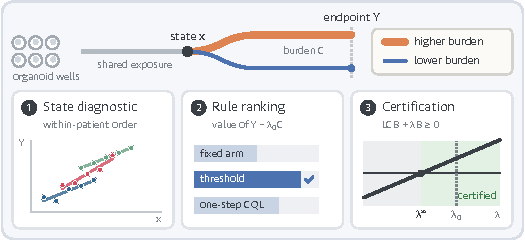
\includegraphics[width=\linewidth]{fig1_overview.pdf}
\caption{Study overview. At a shared checkpoint, each organoid well has a state \(x\), two observed arms of different burden \(C\), and an endpoint \(Y\). The protocol characterizes what the state supports, retains the leading lower-burden rule by the value of \(Y-\lambda_0C\), and certifies it from the critical rate \(\lambda^\ast\).}
\label{fig:overview}
\end{figure}

However, learning a full treatment policy across a trajectory would need patient diversity, repeated decision points, and broad action support beyond what offline policy learning can supply in clinical settings \cite{levine2020, gottesman2019}. A public organoid screen instead presents a single decision point over a handful of patients, where both candidate actions are already observed (Fig.~\ref{fig:overview}). This structure supports off-policy evaluation in its one-step, contextual-bandit form \cite{dudik2011}. We therefore study the de-escalation decision it can support, which uses the state at the decision point to select a shorter or lower-dose regimen that holds final tumor killing within a patient-level non-inferiority margin.

The estimand is the set of decision-point contexts where treatment burden can be reduced while final killing stays within that margin. Burden means exposure duration or dose, together with the cost, side-effect risk, and resource use they carry. We let the margin grow with the burden a rule saves, priced at an exchange rate that the decision context sets. This construction follows the net-benefit reading of cost-effectiveness analysis, where a less effective but less costly option is acceptable once the cost it saves, valued at a stated threshold, outweighs the effect it gives up \cite{stinnett1998, fenwick2001}. Certification therefore returns a threshold rate, above which the lower-burden rule is non-inferior, and we read it against the rate at which full de-escalation breaks even in the data.

A three-stage protocol produces this threshold by characterizing what the decision-point state supports, ranking lower-burden rules by patient-weighted doubly robust value, and certifying the leading rule under a patient-clustered paired bootstrap bound. Data-calibrated simulations check its error control after candidate selection at three to five patients and size the cohort that confirmation requires. The paper contributes the certification protocol with its operating-characteristic audit, an organoid de-escalation benchmark built from a documented search of public data, certified burden-price thresholds for an exposure-duration rule and a dose-intensity rule, and a replication of the frozen protocol on a radiation cohort.\footnote{\url{https://github.com/yingzhe0301-IM/BIBM2026_ooc_rl} holds the code, processed data, and search log.}

\section{Related Work}

\subsection{Organoid Functional Medicine}

Biobanks, prospective drug testing, and imaging readouts connect organoid response with patient treatment response \cite{vlachogiannis2018, ooft2021, spiller2021}. Most of this work measures sensitivity after a fixed exposure, whereas de-escalation needs a shared readout followed by observed lower- and higher-burden actions. Organoid-on-chip and microfluidic platforms create this comparison by varying concentration, combination, sequence, and duration \cite{man2024, schuster2020, wangclevers2025}.

\subsection{Policy Learning, Safe Improvement, and Non-Inferiority}

Dynamic treatment regimes and individualized treatment rules describe decisions that depend on patient state \cite{murphy2003, qian2011}. Offline reinforcement learning extends that idea to data generated by existing treatment choices, where some actions may be sparse or absent, and conservative Q-learning penalizes unsupported actions \cite{levine2020, kumar2020}. Off-policy evaluation contributes doubly robust value estimation, whose point estimates remain fragile in clinical data \cite{dudik2011}. Safe policy improvement responds by returning a new policy only when a high-confidence bound places its performance above that of the baseline. High-confidence policy improvement computes the bound on data held out from the policy search \cite{thomas2015}, baseline bootstrapping keeps the baseline's probability for every action with few logged examples \cite{laroche2019}, and recent work restricts improvement to decision points with enough examples of each action \cite{sharma2025}. All three slices log both arms within every family by design, so the support that these constraints protect is already present, and the remaining risk is sampling error across a few patients. These methods certify a single reward against a fixed tolerance. Our certificate trades two outcomes, endpoint and burden, and reports the range of exchange rates over which the replacement holds.

Empirical welfare maximization and observational policy learning justify optimizing over restricted, deployable rule classes \cite{kitagawa2018, athey2021}, and depth-limited policy trees make such rules readable \cite{zhou2018}. With few patients, a free tree search spends most of the cross-patient information on selecting splits, so we compare a small fixed family of candidate rules and keep trees as audit classes.

Clinical de-escalation also sets a stricter standard than policy ranking alone. Non-inferiority designs trade a bounded efficacy loss for lower burden and certify a lower-burden regimen when its outcome clears a prespecified margin \cite{piaggio2012, iveson2018, grothey2018}. Clinical trials usually fix one accepted margin in advance, whereas net-benefit analysis reports results across a range of willingness-to-trade values \cite{stinnett1998, fenwick2001}. With only a few patients, inference must also respect patient clusters, and standard variance estimates are unreliable in this regime \cite{cameron2015}.

\section{Dataset and Benchmark Construction}
\label{sec:data}

A defensible de-escalation analysis needs three pieces in the same dataset: a decision point with both lower- and higher-burden actions observed, a state measured before that point, and a final efficacy readout afterward. We build three such slices from public organoid experiments. They share the same decision structure but put burden on different axes. Schuster varies how long treatment runs, Spiller varies how much drug is delivered, and Wells varies the radiation dose. Table~\ref{tab:composition} gives the patient-to-well composition of the three slices.

The Schuster slice comes from three pancreatic-cancer organoid lines, each derived from a distinct patient and screened across four chemotherapy families, namely FOLFIRINOX, FOLFIRI, FOLFOX, and Gemcitabine + 5FU \cite{schuster2020}. We use the per-well fluorescence time series of its schedule experiment, which the article releases in its source-data file (sheet Figure~5a--b). Every family is run under two schedules that share a 4-hour exposure window and then split, one arm stopping at the checkpoint and the other continuing to 72 hours, so both arms are observed at a single shared checkpoint. Two fluorescence channels track each well over the window, a propidium-iodide death signal and a matched Caspase apoptosis signal. Raw fluorescence drifts across wells and patients, so every marker is read as the negative-control log-ratio \(\log(x/\bar{x}_{\mathrm{neg}})\), where \(\bar{x}_{\mathrm{neg}}\) is the matched negative-control mean for the same patient, marker, and time point. We keep the two scheduled arms of the four families at the checkpoint and the endpoint, set aside the third, time-modulated schedule, and use negative-control wells only for normalization. This yields 78 well-level episodes, 39 stopping and 39 continuing, each with a complete checkpoint state and final death endpoint. Figure~\ref{fig:checkpoint} shows that wells with higher checkpoint death tend to reach higher final death within each patient.

\begin{table}[t]
\caption{Patient-to-episode composition of the benchmark. Every well, or tracked organoid for Wells, is one episode. Replicates count wells per family and arm, or organoids per arm for Wells, and lists follow the patient order of Table~\ref{tab:cert}.}
\label{tab:composition}
\centering
\footnotesize
\setlength{\tabcolsep}{3.5pt}
\begin{tabular}{@{}llllr@{}}
\toprule
Slice & Families & Replicates & Episodes per patient & Total \\
\midrule
Schuster & 4 each & 2--3, 2--3, 4 & 23 / 23 / 32 & 78 \\
Spiller & 2, 2, 2, 1 & 3 & 12 / 12 / 12 / 6 & 42 \\
Wells & 1 each & 33--111 & 193 / 184 / 155 / 70 / 106 & 708 \\
\bottomrule
\end{tabular}
\end{table}

\begin{figure}[t]
\centering
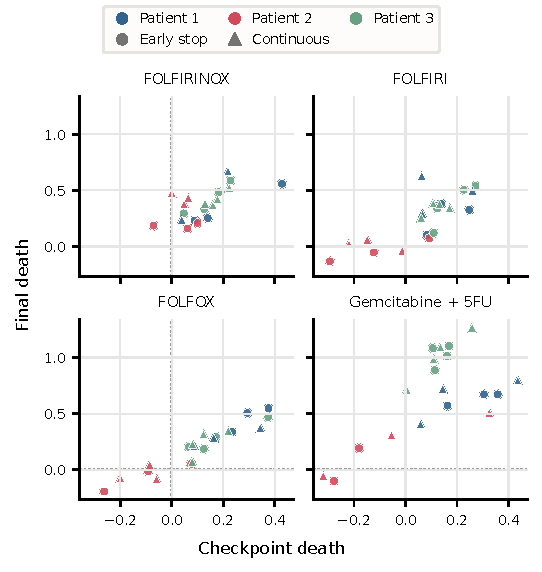
\includegraphics[width=\linewidth]{fig2_checkpoint_scatter.pdf}
\caption{Family-wise checkpoint geometry in Schuster. Checkpoint and final propidium-iodide signals are shown as negative-control log-ratios. Color denotes patient and marker denotes action arm.}
\label{fig:checkpoint}
\end{figure}

The Spiller slice comes from four colorectal organoid lines, each from a distinct patient \cite{spiller2021}. We use the organoid-level table that the authors release in their public code repository\footnote{\url{https://github.com/eitm-org/organoid_drug_response}, file \texttt{data/consolidated.csv}.}. Brightfield images track organoids over seven days, and a machine-learning classifier labels each organoid as live or dead before wells are summarized by dead fraction. Here the action is dose. Irinotecan is given at 20 or 40~\si{\micro\molar} and oxaliplatin at 2 or 20~\si{\micro\molar} for the same seven days, so burden is the concentration-time of the assigned arm and any saving comes from lower concentration. We keep the lines screened at both doses of a contrast, four for irinotecan and three for oxaliplatin, which gives 42 well-level episodes with three replicates per patient, family, and arm and no missing readings. Both arms start at day~0, so the day-0 dead fraction is the only reading that precedes the action. We use it as the state and the day-7 dead fraction as the endpoint. Figure~\ref{fig:spiller} shows the dose arms overlapping before dosing begins and widening toward the endpoint.

\begin{figure}[t]
\centering
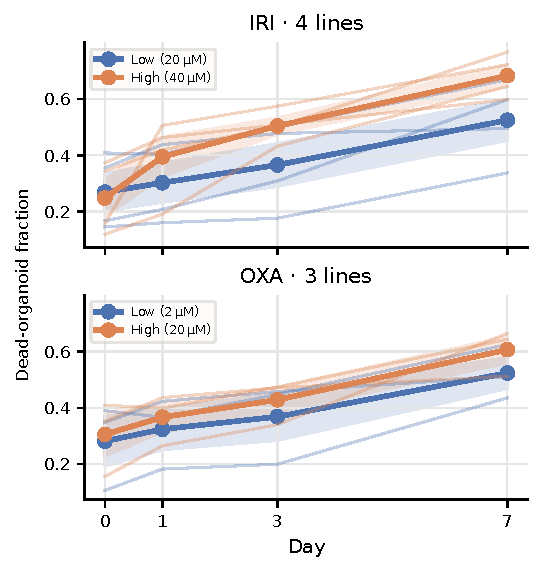
\includegraphics[width=\linewidth]{fig3_spiller_trajectories.pdf}
\caption{Spiller dose-arm response trajectories. Well-level dead-organoid fraction is shown across days for the retained low- and high-dose arms.}
\label{fig:spiller}
\end{figure}

The Wells slice comes from organoids of five luminal breast cancers, each from a distinct patient and cultured without passaging \cite{wells2026}. We use the per-organoid tables released with the authors' code\footnote{\url{https://github.com/JanesLab/WellsCJ_OrganoSeg2}, archive \texttt{Figure 6/excelFilesZip.zip}.}. Each patient's organoids receive 0, 5, or 30~Gy in five daily fractions, one well per dose, and a caspase-3/7 reporter loaded on the first irradiation day is imaged before the first fraction and then through day~14. The 30~Gy course mirrors accelerated partial breast irradiation, and the 5~Gy arm is its de-escalation. Each tracked organoid is one episode. Its state is the reporter reading before the first fraction, its endpoint is the reading at day~14, both as log-ratios to the same patient's 0~Gy organoids as in Schuster, and burden is the total dose. Keeping organoids read at both times gives 708 episodes. Each arm occupies one well per patient, so well effects within a patient are confounded with the arm. We added this slice during revision and analyze it with the protocol unchanged.

We searched public resources for datasets with this structure on 17 and 18 October 2026. A dataset qualified when it held tumor organoids from at least three patients, two burden levels of one treatment within each patient, a per-well state read before the arms diverge together with an endpoint on the same wells, and well-level data released without request. The search covered titles and abstracts in Europe PMC, which indexes PubMed and the major preprint servers, full texts that name a data repository, every article citing Schuster or Spiller, and Zenodo, Figshare, Dryad, the BioImage Archive, BioStudies, the Image Data Resource, and GitHub. Screening 3597 unique records by title, abstract, and description left 242 records from 193 studies for assessment against the full text and the released files. Four studies met all four conditions, namely Schuster, Spiller, Wells, and a 2026 preprint from the Spiller group that tracks colorectal organoids from six patients through eight doses of SN-38 and 5-FU \cite{kim2026}. Four more ran the required design with released files whose per-well content we could not confirm, and eighteen ran it with data available only on request. Public per-well data, more than experimental design, therefore limit this benchmark. Wells enters the benchmark as a third burden axis, and the preprint, which repeats the Spiller design with a dose series, is the next replication cohort. The query strings and the screening log are released with our code.

\section{Staged Evaluation Protocol}

All three stages use a shared patient-level scaffold. The unit of analysis is a well \(i\), or a tracked organoid for Wells, from patient \(p\), the cluster held out and resampled throughout. Each well has a state \(x_i\) measured before the action, a final endpoint \(Y_i\), a binary logged action \(a_i\), and a treatment burden \(C_i\). Higher \(Y_i\) means more tumor death, the efficacy we preserve, while \(a_i\) indicates the lower- or higher-burden arm. A policy \(\pi\) maps a state to an action, with endpoint value \(V_Y(\pi)\) and burden \(V_C(\pi)\). We estimate endpoint values doubly robustly, using a ridge outcome model \(\hat q(x,a)\) on state and family and a family-level propensity \(e(a\mid\mathrm{family})\). Both nuisance functions are fit on patients outside the held-out one.

Policy value is the mean of patient-level averages rather than a well-level mean. With on-policy weight \(w_i=\mathbf 1\{a_i=\pi(x_i)\}/e(a_i\mid\mathrm{family}_i)\), endpoint value is estimated by
\begin{equation}
\hat V_Y(\pi)=\frac{1}{G}\sum_{p=1}^{G}\frac{1}{n_p}\sum_{i:p_i=p}\!\Bigl[\hat q(x_i,\pi(x_i))+w_i\bigl(Y_i-\hat q(x_i,a_i)\bigr)\Bigr],
\end{equation}
where \(G\) is the patient count and \(n_p\) is the number of held-out wells for patient \(p\). This definition prevents patients with more retained wells from dominating the target. Burden values use the same patient-level averaging.

The experimental design supplies the identifying assumptions. Positivity holds by construction, since both arms are observed in every family and candidate rules act only where both actions are observed. The family-level propensity \(e(a\mid\mathrm{family})\) is a known design proportion, so once family is fixed the logged arm is unconfounded with a well's endpoint, and the state enters \(\hat q(x,a)\) only to sharpen the estimate. Biological transfer from organoid to patient remains an assumption for prospective validation.

\subsection{Stage 1: State Diagnostic}

Stage 1 characterizes what the decision-point state can support before any policy is ranked. We regress \(Y_i\) on \(x_i\) under leave-one-patient-out and read two quantities. Mean absolute error (MAE) measures level, and the within-patient Spearman correlation \(\rho\) between prediction and endpoint measures ordering. We also compute the rank correlation between state and endpoint inside each patient, family, and arm cell, where the design is held fixed. A state that orders wells within patients supports rules that act within a patient, and a state without that order supports only rules that act between patients or families. Per-patient \(R^2\) is negative for every model on the chemotherapy slices, because it charges the unpredictable patient-level offset to the ordering, so we report \(\rho\) in its place.

\subsection{Stage 2: Burden-Aware Candidate Discovery}

Stage 2 turns the state into ranked lower-burden candidates. Let \(\lambda\) be the exchange rate, the endpoint loss accepted for one unit of burden saved. Each well receives the burden-adjusted reward
\begin{equation}
R_{\lambda}=Y-\lambda C,
\end{equation}
and policies are ranked by the patient-weighted doubly robust value of \(R_\lambda\).

The decision context chooses \(\lambda\), so each slice reports it relative to its own reference rate. Let \(\pi_{\mathrm{low}}\) be the fully de-escalated arm and \(\pi_0\) the high-burden baseline. The reference rate is the endpoint gap divided by the burden gap between the two fixed arms,
\begin{equation}
\lambda_0=\frac{|V_Y(\pi_{\mathrm{low}})-V_Y(\pi_0)|}{|V_C(\pi_{\mathrm{low}})-V_C(\pi_0)|}.
\end{equation}
Here \(\lambda_0\) is the empirical break-even price, the endpoint traded for one unit of burden when the population moves from baseline to full de-escalation. It uses only the two fixed arms and is therefore independent of every candidate policy and of \(\lambda\). A rule that de-escalates a random share of wells loses endpoint and saves burden in the same proportion, so its point margin at \(\lambda_0\) is exactly zero. A positive point margin at \(\lambda_0\) therefore means that a rule selects wells for de-escalation better than chance. We report results on the scale-free axis \(\lambda/\lambda_0\) and read them against a band \(\Lambda=[0.5,2]\lambda_0\), a convention spanning a factor of two around the break-even. For Schuster, burden is exposure time and \(\lambda_0=8.6\times10^{-4}\) log-ratio units per hour saved. For Spiller, burden is concentration-time and \(\lambda_0=3.6\times10^{-5}\) dead fraction per \si{\micro\molar\hour} saved. Because \(\lambda_0\) comes from the same patients, we also recompute it with each patient left out.

To limit selection at this sample size, Stage 2 retains one of three prespecified lower-burden classes, namely the fixed low-burden arm, family-specific thresholds on the state, and one-step conservative Q-learning (CQL). A family-specific threshold learns one cutpoint and direction within each family by inverse-propensity value, with ties broken toward lower burden, which keeps it inside a restricted rule class in the sense of empirical welfare maximization \cite{kitagawa2018}. The CQL candidate scores each action with a linear function of the standardized state, family indicators, and an intercept. In the contextual-bandit form of \cite{kumar2020}, the two scores are fit to the burden-adjusted reward at \(\lambda_0\) with penalty weight \(\eta=1\), fixed at implementation and left untuned. The penalty discourages actions poorly supported by the logged assignments, and \(\eta=0\) recovers plain one-step Q-learning, which fits one linear model per arm and is therefore the T-learner of treatment-effect estimation with linear base learners \cite{kunzel2019}. Every candidate is fit on the other patients and evaluated on the held-out one, and Stage 2 retains the class with the highest patient-weighted value of \(R_{\lambda_0}\). Audit classes pass through the same evaluation and certification and stay out of retention. They comprise a family-only rule that picks the better fixed arm per family, CQL without the state, CQL at \(\eta\in\{0,0.1,10\}\), a T-learner with a 200-tree random forest per arm, and depth-limited doubly robust policy trees \cite{athey2021, zhou2018} with at least four wells and both actions in every leaf.

\subsection{Stage 3: Conservative Replacement Certification}

Stage 3 issues a preclinical certificate, which states that the retained candidate can replace the baseline inside a patient-level non-inferiority margin on the organoid endpoint. Two quantities define the replacement contrast. The endpoint contrast \(\delta_\pi=V_Y(\pi)-V_Y(\pi_0)\) is the endpoint change from switching, and the burden saving \(B_\pi=V_C(\pi_0)-V_C(\pi)\) is the burden the switch removes on the observed wells. For any de-escalating rule, \(B_\pi\ge 0\). Priced at \(\lambda\), this saving permits an endpoint loss \(m_\pi=\lambda B_\pi\). The candidate certifies when its conservative endpoint contrast clears that allowance,
\begin{equation}
M(\lambda)=LCB_{1-\alpha}(\delta_\pi)+\lambda B_\pi\ge 0,
\end{equation}
where \(LCB_{1-\alpha}(\delta_\pi)\) is the one-sided lower confidence bound on \(\delta_\pi\), one-sided because only an endpoint loss can violate non-inferiority. The margin \(M(\lambda)\) rises with \(\lambda\), so a higher price of burden can only help a burden-saving rule. The certificate therefore reduces to a single threshold, the critical exchange rate
\begin{equation}
\lambda^\ast(\pi)=\frac{-LCB_{1-\alpha}(\delta_\pi)}{B_\pi},
\end{equation}
the lowest price at which the rule certifies. The rate \(\lambda^\ast\) is computed without \(\lambda_0\), which enters the analysis only as the price in the Stage 2 training reward and as the unit for reading \(\lambda^\ast\). We report \(\lambda^\ast/\lambda_0\). A ratio below one means the rule clears the bar even below the data's break-even, and a ratio above one means it needs a context that values burden reduction more than the data's own tradeoff.

The certificate uses a paired two-stage cluster bootstrap with \(\alpha=0.05\). It resamples patients with replacement and then wells within each sampled patient, keeping each well's candidate and baseline values paired, and takes the 5\% quantile of the patient-weighted contrast over 50,000 resamples. Within a patient, wells are drawn regardless of family or arm. Retaining one of three classes is a selection step. Safe policy improvement separates selection from the safety test by holding out data \cite{thomas2015}, which with three to five patients would leave one to three patients for the test. We therefore certify on all patients, add an adjusted certificate at level \(0.05/3\), and check the error after selection by simulation (Section~\ref{sec:stress}). A wild-cluster screen flips Rademacher signs on the patient-level contrasts and enumerates all \(2^G\) patterns. Its attainable one-sided levels are multiples of \(2^{-G}\), namely 0.125 for Schuster, 0.0625 for Spiller, and 0.031 for Wells, so it serves as a screen and the paired bound serves as the certificate. Outcome models are ridge regressions with unit penalty on the standardized state and one-hot family, one per logged action, and the propensity is clipped to \([0.05,0.95]\). Threshold search scans 21 within-family quantiles of the state from 5\% to 95\% and requires two wells on each side of a cut.

\section{Results}

\subsection{Stage 1: What the State Supports}

On Schuster, the checkpoint carries within-patient order. Adding checkpoint death lowers MAE from 0.266 to 0.189 and raises the within-patient rank correlation from 0.56 to 0.75 (Table~\ref{tab:p1}). Inside fixed patient, family, and arm cells, checkpoint and final death have a mean rank correlation of 0.60, positive in 18 of 22 cells. The matched apoptosis channel adds nothing beyond death, so later stages carry checkpoint death with family. On Spiller, the pre-treatment state carries no such signal. It raises MAE from 0.104 to 0.117, leaves \(\rho\) near 0.60, and has a mean within-cell rank correlation of \(-0.11\). A Spiller rule can therefore act only between patients or families, and we read its certificate as evidence about that coarser structure.

\begin{table}[t]
\caption{Stage~1 leave-one-patient-out endpoint prediction. MAE measures level, and \(\rho\), the within-patient Spearman correlation between prediction and endpoint, measures ordering. The state is checkpoint death for Schuster, pre-treatment dead fraction for Spiller, and the pre-irradiation caspase reading for Wells. The second channel is apoptosis for Schuster and organoid size for Wells.}
\label{tab:p1}
\centering
\footnotesize
\setlength{\tabcolsep}{4pt}
\begin{tabular}{@{}lrrrrrr@{}}
\toprule
 & \multicolumn{2}{c}{Schuster} & \multicolumn{2}{c}{Spiller} & \multicolumn{2}{c}{Wells} \\
\cmidrule(lr){2-3}\cmidrule(lr){4-5}\cmidrule(l){6-7}
Ridge features & MAE & \(\rho\) & MAE & \(\rho\) & MAE & \(\rho\) \\
\midrule
Family + arm & 0.266 & 0.56 & 0.104 & 0.60 & 0.106 & 0.08 \\
+ state & \textbf{0.189} & \textbf{0.75} & 0.117 & 0.61 & 0.106 & 0.17 \\
+ second channel & 0.192 & 0.71 & --- & --- & 0.081 & 0.63 \\
\bottomrule
\end{tabular}
\end{table}

\subsection{Certification of the Retained Rules}

Stage 2 retains the family-specific threshold rule on Schuster and the one-step CQL rule on Spiller. Re-deriving candidates across \(\Lambda\) keeps both retentions, except at \(2\lambda_0\) on Spiller, where the fixed low-dose arm takes the lead. Table~\ref{tab:cert} reports their certification next to the other prespecified classes and the radiation slice, and Fig.~\ref{fig:decision} draws the margin of each chemotherapy rule along the \(\lambda/\lambda_0\) axis.

\begin{table*}[t]
\caption{Certification of the prespecified lower-burden classes against the higher-burden baseline. Burden saved is in hours for Schuster, in \si{\micro\molar\hour} for Spiller, and in Gy for Wells. Per-patient \(\Delta\) lists the patient-level endpoint contrasts that the clustered bounds resample. Critical ratios are given for the wild-cluster screen, the paired certificate, and the certificate adjusted for retaining one of three classes. Retained rules in bold.}
\label{tab:cert}
\centering
\footnotesize
\setlength{\tabcolsep}{3pt}
\begin{tabular*}{\textwidth}{@{\extracolsep{\fill}}llrrlrrrr@{}}
\toprule
 & & & & & & \multicolumn{3}{c}{\(\lambda^\ast/\lambda_0\)} \\
\cmidrule(l){7-9}
Task & Policy & \makecell[r]{Burden\\saved} & \makecell[r]{\(\Delta\)\\endpoint} & Per-patient \(\Delta\) & \makecell[r]{Paired\\LCB} & Screen & Certificate & Adjusted \\
\midrule
Schuster & Always stop & 68.0 (94\%) & \(-0.059\) & \(-0.141\) / \(-0.058\) / \(+0.024\) & \(-0.169\) & 1.94 & 2.89 & 3.41 \\
 & \textbf{Family-specific threshold} & 26.3 (36\%) & \(+0.014\) & \(-0.034\) / \(+0.035\) / \(+0.039\) & \(-0.044\) & 0.80 & \textbf{1.95} & 2.69 \\
 & One-step CQL & 27.8 (39\%) & \(-0.040\) & \(-0.120\) / \(+0.035\) / \(-0.036\) & \(-0.127\) & 3.90 & 5.30 & 6.51 \\
\midrule
Spiller & Always low dose & 3234 (59\%) & \(-0.115\) & \(-0.303\) / \(-0.055\) / \(-0.049\) / \(-0.055\) & \(-0.226\) & 1.81 & 1.96 & 2.25 \\
 & Family-specific threshold & 938 (17\%) & \(-0.047\) & \(-0.111\) / \(-0.045\) / \(-0.033\) / \(0.000\) & \(-0.100\) & 2.36 & 2.98 & 3.46 \\
 & \textbf{One-step CQL} & 1386 (25\%) & \(-0.003\) & \(0.000\) / \(+0.019\) / \(-0.032\) / \(0.000\) & \(-0.051\) & 0.36 & \textbf{1.02} & 1.36 \\
\midrule
Wells & \textbf{Always low dose} & 25.0 (83\%) & \(+0.029\) & \(+0.068\) / \(+0.007\) / \(+0.046\) / \(+0.050\) / \(-0.027\) & \(-0.003\) & 0.00 & \textbf{0.10} & 0.41 \\
 & Family-specific threshold & 24.6 (82\%) & \(+0.027\) & \(+0.059\) / \(+0.007\) / \(+0.046\) / \(+0.050\) / \(-0.027\) & \(-0.003\) & 0.00 & 0.12 & 0.45 \\
 & One-step CQL & 24.0 (80\%) & \(+0.022\) & \(+0.038\) / \(+0.007\) / \(+0.043\) / \(+0.051\) / \(-0.027\) & \(-0.006\) & 0.00 & 0.21 & 0.50 \\
\bottomrule
\end{tabular*}
\end{table*}

On Schuster, the threshold rule continues wells whose checkpoint death is low for their family and stops the rest. It saves 26 of the 72 baseline hours while the patient-weighted endpoint rises by 0.014. The per-patient contrasts trace the uncertainty to the one patient whose endpoint falls. The paired bound places the endpoint loss at no more than 0.044, so the rule certifies once a context accepts that loss for 26 fewer hours of exposure, which happens at \(1.95\lambda_0\). The wild screen passes the rule at \(0.80\lambda_0\), below the break-even.

On Spiller, the CQL rule keeps the high dose for the two lines with a low baseline dead fraction of 0.14 and lowers it for most wells of the two lines at 0.36 and 0.39. It removes a quarter of dose burden with an endpoint change of \(-0.003\). The paired bound allows a loss of 0.051 for that saving, so the rule certifies from \(1.02\lambda_0\), just above the break-even. Its value comes from the patient level. Full de-escalation costs 0.30 in final dead fraction for line 12415 and about 0.05 for the other three lines, and the rule keeps 12415 on the high dose. This between-patient mechanism is consistent with Stage 1 and rests on four lines.

\begin{figure}[t]
\centering
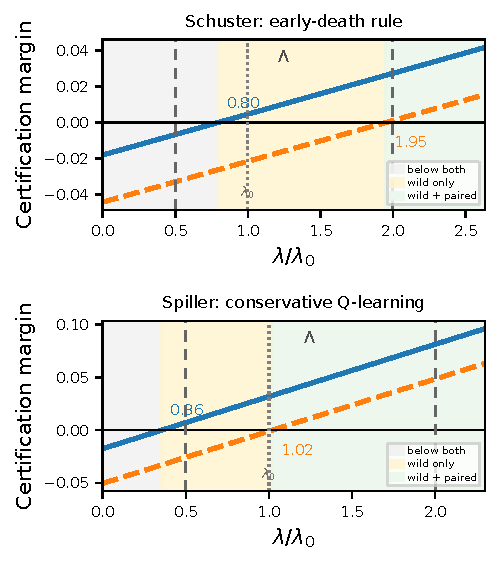
\includegraphics[width=\linewidth]{fig4_certification_curve.pdf}
\caption{Certification curves of the retained chemotherapy rules. The certification margin \(M(\lambda)\) is plotted against \(\lambda/\lambda_0\) for each rule. The solid line is the wild-cluster screen and the dashed line is the paired certificate. The three shaded bands, from left to right, mark where neither reading certifies, where only the screen certifies, and where the certificate holds.}
\label{fig:decision}
\end{figure}

\subsection{Audit Classes and Sensitivity}

Table~\ref{tab:audit} compares the retained rules with the audit classes. On Schuster, every state-free comparator certifies later than the threshold rule. The family-only rule and CQL without the state need \(3.34\lambda_0\) and \(3.35\lambda_0\), against \(1.95\lambda_0\) for the threshold rule, which shows that the checkpoint carries the Schuster result beyond the family structure. On Spiller, the same state-free rules save only 15\% of the burden. The more flexible learners trail the retained rules on both slices. The random-forest T-learner, which estimates each well's treatment effect, loses the most endpoint of any audit class, and depth-limited trees certify only above \(2.7\lambda_0\).

\begin{table}[t]
\caption{Audit classes, fit and certified like the prespecified classes on held-out patients and excluded from retention. Columns give the burden saved as a share of the baseline, the endpoint contrast \(\Delta\) against the baseline, the certificate's critical ratio, and the share of wells whose action matches the prespecified CQL rule at \(\eta=1\).}
\label{tab:audit}
\centering
\footnotesize
\begin{tabular}{@{}lrrrr@{}}
\toprule
Audit class & Saved & \(\Delta\) & \(\lambda^\ast/\lambda_0\) & Agreement \\
\midrule
\multicolumn{5}{@{}l}{\emph{Schuster}} \\
Family only & 64\% & \(-0.035\) & 3.34 & 0.67 \\
CQL without state & 48\% & \(-0.032\) & 3.35 & 0.67 \\
One-step Q, \(\eta=0\) & 70\% & \(-0.046\) & 3.44 & 0.65 \\
CQL, \(\eta=0.1\) & 61\% & \(-0.037\) & 3.59 & 0.74 \\
CQL, \(\eta=10\) & 46\% & \(-0.023\) & 3.26 & 0.71 \\
T-learner, forest & 41\% & \(-0.050\) & 4.97 & 0.67 \\
Policy tree, depth 1 & 60\% & \(-0.042\) & 3.77 & 0.60 \\
Policy tree, depth 2 & 51\% & \(-0.046\) & 4.42 & 0.65 \\
\midrule
\multicolumn{5}{@{}l}{\emph{Spiller}} \\
Family only & 15\% & \(-0.076\) & 6.85 & 0.21 \\
CQL without state & 15\% & \(-0.076\) & 6.86 & 0.21 \\
One-step Q, \(\eta=0\) & 43\% & \(-0.097\) & 2.63 & 0.67 \\
CQL, \(\eta=0.1\) & 43\% & \(-0.097\) & 2.63 & 0.67 \\
CQL, \(\eta=10\) & 30\% & \(-0.026\) & 1.23 & 0.60 \\
T-learner, forest & 40\% & \(-0.108\) & 2.90 & 0.62 \\
Policy tree, depth 1 & 36\% & \(-0.097\) & 3.06 & 0.55 \\
Policy tree, depth 2 & 39\% & \(-0.089\) & 2.77 & 0.69 \\
\bottomrule
\end{tabular}
\end{table}

The CQL penalty shapes the Spiller result. Plain one-step Q-learning and \(\eta=0.1\) learn the same rule, which agrees with the \(\eta=1\) rule on 67\% of wells and certifies only from \(2.63\lambda_0\). At \(\eta=10\), the rule changes again, agrees on 60\% of wells, and certifies from \(1.23\lambda_0\). The Spiller result therefore depends on the penalty, while on Schuster CQL trails the threshold rule at every penalty.

Further checks bound the reading. The adjusted certificate moves the critical ratio to \(1.36\lambda_0\) for Spiller, inside \(\Lambda\), and to \(2.69\lambda_0\) for Schuster, beyond it. Leaving out one patient at a time scales \(\lambda_0\) by 0.42 to 1.10 on Schuster and by 0.51 to 1.19 on Spiller. The Spiller critical ratio of 1.02 lies inside this range, so its position relative to the break-even depends on which patients set the reference. The burden saving also varies under resampling, with 90\% intervals of 10 to 42 hours for the Schuster rule and 0 to 2632~\si{\micro\molar\hour} for the Spiller rule. Resampling it jointly with the endpoint lowers the critical ratios to \(1.81\lambda_0\) and \(1.01\lambda_0\), so the fixed-saving certificate is the conservative reading. Across threshold grids of 11, 21, and 41 quantiles and minimum leaf sizes of 3, 4, and 6 wells, Stage 2 retains the same classes, the coarsest grid moves the Schuster rule to \(2.27\lambda_0\), and the chemotherapy trees stay above \(2.6\lambda_0\).

\subsection{Replication on the Radiation Slice}

Applied unchanged to Wells, the protocol meets data in which the higher burden buys little. The pre-irradiation reporter reading orders organoids weakly, raising the within-patient \(\rho\) from 0.08 to 0.17 with no gain in MAE, while organoid size raises it to 0.63 (Table~\ref{tab:p1}). Stage 2 retains the fixed 5~Gy arm at every price in \(\Lambda\). The 30~Gy course adds no apoptosis over 5~Gy in four of five patients, so full de-escalation gains 0.029 on average, and \(\lambda_0=1.2\times10^{-3}\) per Gy measures the size of that gain. The paired bound allows a loss of at most 0.003 for 25~Gy less radiation, which certifies the 5~Gy arm from \(0.10\lambda_0\), or \(1.2\times10^{-4}\) per Gy, and from \(0.41\lambda_0\) after adjustment. Every audit class certifies by \(0.26\lambda_0\). The source study reaches the same reading through survival analysis, with 5~Gy inducing caspase-positive organoids at the same rate as 30~Gy in the two most responsive cases \cite{wells2026}. The certificate thus finds no organoid evidence for the extra 25~Gy on this endpoint.

\subsection{Synthetic Operating-Characteristic Stress Test}
\label{sec:stress}

To address the concern that three to five patients are too few to trust a certificate, we audit the procedure itself on known-truth simulations calibrated to each slice \cite{morris2019,franklin2014}. The synthetic data match the observed patient counts, wells per patient, endpoint scale, and the between- and within-patient standard deviations of the retained rule's contrast, 0.041 and 0.285 for Schuster and 0.021 and 0.190 for Spiller. We set the true margin as \(\Delta=E[Z]\) for the margin-adjusted contrast \(Z=\delta+\lambda B\), with negative, zero, and positive values denoting inferior, boundary, and non-inferior rules. Every dataset passes through the same wild-cluster and paired bounds with 500 resamples. A well-level study reruns the full doubly robust estimator, and a selection study reruns discovery, retention, and certification on null data where every lower-burden rule sits at its boundary.

\begin{figure}[t]
\centering
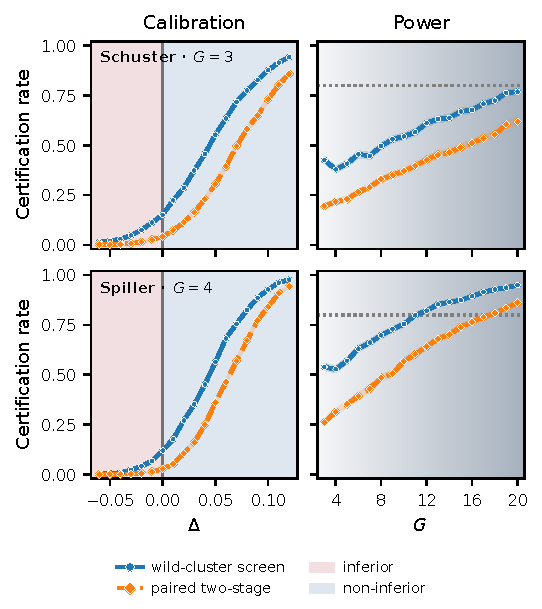
\includegraphics[width=\linewidth]{fig5_stress.pdf}
\caption{Data-calibrated operating characteristics (3000 trials per point; 95\% Monte Carlo bands). Left: certification rate against the true margin \(\Delta\), shaded inferior and non-inferior. Right: power against patient count \(G\) at the observed effect, with the 0.8 reference marked.}
\label{fig:stress}
\end{figure}

Figure~\ref{fig:stress} reports calibration and power. At the boundary, the paired certificate passes 4.2\% of Schuster and 2.8\% of Spiller trials, and it passes a rule that is 0.02 inferior in at most 1.5\% of trials. The wild screen passes 15\% and 12\% at the boundary, which is why it serves only as a screen. The paired level depends on between-patient heterogeneity. When the between-patient share of variance rises to 0.30, the boundary rate grows to 12\% for Schuster and 9\% for Spiller. Selection also costs level. Retaining the best of three classes on null data raises the paired rate of any certification to 8.8\% and 5.7\%, and the adjusted certificate brings it to 4.8\% and 2.5\%. The well-level study shows a doubly robust contrast with bias below 0.003 and paired coverage of 0.97 and 0.98. At the Wells geometry, with five patients, the paired certificate passes 5.7\% of boundary trials and 1.5\% of null trials after selection. Power at the observed effects is 0.20 and 0.31 at the available patient counts. It reaches 0.8 at 18 patients for the Spiller effect and stays at 0.62 at 20 patients for the Schuster effect, which sizes a confirmatory cohort.

\section{Discussion}

The protocol turns a de-escalation question into a burden-price threshold. For a laboratory or translational team, \(\lambda^\ast\) states how much endpoint loss per unit of burden saved a context must accept before the evidence supports the switch. On these data, the exposure rule certifies whenever a loss of 0.044 in final log-ratio death is acceptable for 26 fewer hours of exposure, and the dose rule whenever a loss of 0.051 in dead fraction is acceptable for a quarter less dose. Net-benefit analysis in health economics rests on the same structure \cite{stinnett1998, fenwick2001}, so the threshold can come from the kind of deliberation that sets a willingness-to-pay value.

These certificates are preclinical. The endpoints are organoid readouts of tumor-cell death, which differ from patient survival, tumor control, toxicity, and quality of life. Burden enters only as exposure duration, concentration-time, or radiation dose, because the public screens record no adverse events or costs. The framework accepts any per-arm burden measure without change, so a richer burden scale is a matter of data. We therefore present the chemotherapy rules and the radiation finding as replication hypotheses for new organoid cohorts and present \(\lambda^\ast\) as a tool for prioritizing those experiments.

Sample size remains the binding limit. Three to five patients give the certificate low power even when the effect is real, and its level holds only while between-patient heterogeneity stays near the small values these patients show. The well-level and selection simulations also hold the treatment effect fixed across patients, while the observed cost of full de-escalation varies widely between patients, so their rates are optimistic. The Spiller rule acts between patients on a pre-treatment state, so its evidence rests on four lines and on one line in particular. The power analysis turns these limits into a concrete target, about 18 patients for an effect of the Spiller size.

The decision to lower a patient's treatment remains with those who answer for the patient, who weigh tolerance for de-escalation, the oncologist's judgment, institutional risk standards, and liability for any efficacy lost, and certification informs that decision.

\section*{Acknowledgment}

Claude (Anthropic) assisted with developing the analysis code, refactored it for the public release, assisted with figure design, and checked the grammar of the manuscript. Claude agents screened the records of the dataset search in Section~\ref{sec:data} against the written criteria released with the code.

\bibliographystyle{IEEEtran}
\bibliography{refs}

\end{document}
